\chapter{Preliminaries}




\section{Multivariate Calculus}
Let $f\colon\R^n\to\R$ be a function with all partial derivatives existing and being continuous. The \textit{gradient} of $f$ is
\begin{equation*}
\nabla f(\bm{a})=\left(\frac{\partial f(\bm{a})}{\partial x_1},\dots,\frac{\partial f(\bm{a})}{\partial x_n}\right).
\end{equation*}
We write $\nabla_{\bm{x}} f$ or simply $\nabla f$.
% For our purpose we can allow finitely many points where the partial derivatives do not exist -- there we can define them arbitrarily.
To compute derivative of a composition of two or more functions \textit{chain rule} is used. Suppose $g\colon\R^m\to\R^n$ and $z=f(g(\bm{x}))$, then
\begin{equation*}
\frac{\partial z}{\partial x_i}=\sum\limits_{j=1}^n\frac{\partial z}{\partial g(\bm{x})_j}\frac{\partial g(\bm{x})_j}{\partial x_i}\quad\mathrm{or\ in\ vector\ form}\quad\nabla_{\bm{x}}z=\left(\frac{\partial g(\bm{x})}{\partial\bm{x}}\right)^\top\nabla_{g(\bm{x})}z
\end{equation*}
where $\frac{\partial g(\bm{x})}{\partial\bm{x}}$ is the Jacobian matrix.

Given a function $f\colon\R^n\to\R$ we may ask where are its local (or global) minima. For `easy' functions it can be computed analytically, for the most functions however analytical solution is impossible and we therefore introduce numerical method called \textit{gradient descent}. We start with arbitrary point $\bm{x}\in \R{^n}$ and repeat until convergence or certain number of steps:
\begin{equation*}
\bm{x}=\bm{x}-\alpha\nabla_{\bm{x}}f(\bm{x})
\end{equation*}
where $\alpha$ is the step size also called learning rate. Note that the algorithm does not have to converge even for convex functions such as $x^2$ since it can `jump' around $x=0$ indefinitely due to bad value of $\alpha$.
Also if the algorithm converges we are not guaranteed to find the global minimum, we can even be arbitrary far from it. However in machine learning this algorithm with minor modifications is widely used usually producing good-enough minima.

\section{Neural Networks}
Artificial feedforward neural network is a machine learning model capable of learning its parameters $\bm{\theta}$ such that given input $\bm{x}$ it predicts output $\bm{y}=f(\bm{x};\bm{\theta})$. The network is composed of smaller units called neurons defined as
\begin{equation*}
h_i=f\left(\sum_{j}w_{i,j}x_j\right)
\end{equation*}
where $h_i$ is output of $i$\textsuperscript{th} neuron, $x_j$ are its inputs and $f$ is nonlinear function such as $1/(1+e^{-x})$ or $\max(0, x)$. Usually we group neurons into layers and therefore we write $\bm{h}=f(W\bm{x})$ where $W\in\R^{\dim(\bm{h})\times\dim(\bm{x})}$. Simple feedforward neural network with one `hidden' layer can be seen in Figure \ref{}. Such basic network can approximate any continuous functions given there is enough neurons in the hidden layer~\cite{HORNIK}. However the number of neurons can be arbitrary big and empirically networks with more hidden layers usually achieve better results with the same number of neurons.

\todo{Neural Network definition and training}
Convolutional layers have significantly less parameters but are slow to compute using CPU but using GPUs results in exponential speedup.



\begin{tikzpicture}[
init/.style={
	draw,
	circle,
	inner sep=2pt,
	font=\Huge,
	join = by -latex
},
squa/.style={
	draw,
	inner sep=2pt,
	font=\Large,
	join = by -latex
},
start chain=2,node distance=13mm
]
\node[on chain=2] 
(x2) {$x_2$};
\node[on chain=2,join=by o-latex] 
{$w_2$};
\node[on chain=2,init] (sigma) 
{$\displaystyle\Sigma$};
\node[on chain=2,squa,label=above:{\parbox{2cm}{\centering Activate \\ function}}]   
{$f$};
\node[on chain=2,label=above:Output,join=by -latex] 
{$y$};
\begin{scope}[start chain=1]
\node[on chain=1] at (0,1.5cm) 
(x1) {$x_1$};
\node[on chain=1,join=by o-latex] 
(w1) {$w_1$};
\end{scope}
\begin{scope}[start chain=3]
\node[on chain=3] at (0,-1.5cm) 
(x3) {$x_3$};
\node[on chain=3,label=below:Weights,join=by o-latex] 
(w3) {$w_3$};
\end{scope}
\node[label=above:\parbox{2cm}{\centering Bias \\ $b$}] at (sigma|-w1) (b) {};

\draw[-latex] (w1) -- (sigma);
\draw[-latex] (w3) -- (sigma);
\draw[o-latex] (b) -- (sigma);

\draw[decorate,decoration={brace,mirror}] (x1.north west) -- node[left=10pt] {Inputs} (x3.south west);
\end{tikzpicture}


\tikzset{%
	every neuron/.style={
		circle,
		draw,
		minimum size=1cm
	},
	neuron missing/.style={
		draw=none, 
		scale=4,
		text height=0.333cm,
		execute at begin node=\color{black}$\vdots$
	},
}

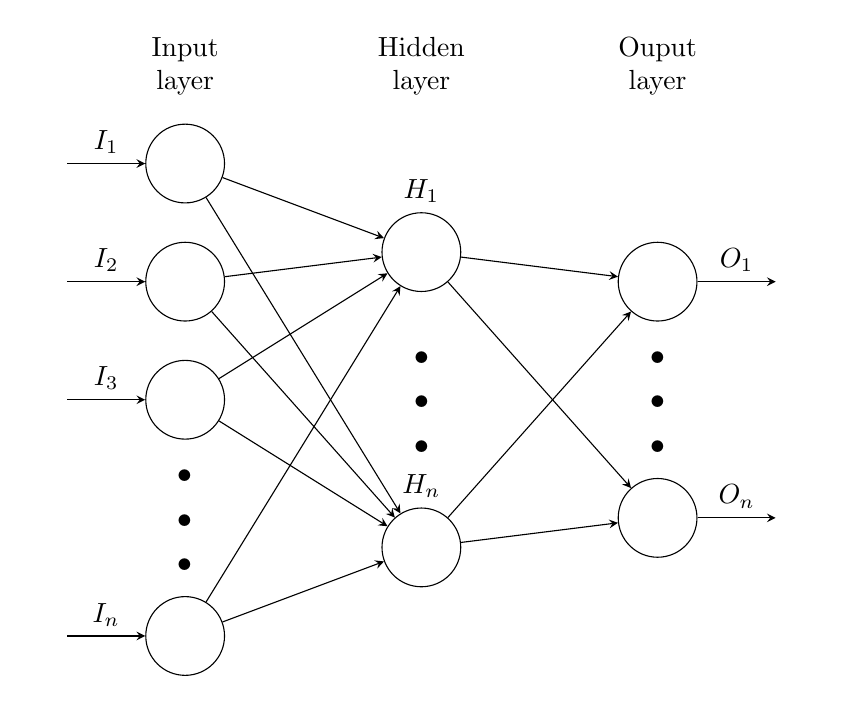
\begin{tikzpicture}[x=1.5cm, y=1.5cm, >=stealth]

\foreach \m/\l [count=\y] in {1,2,3,missing,4}
\node [every neuron/.try, neuron \m/.try] (input-\m) at (0,2.5-\y) {};

\foreach \m [count=\y] in {1,missing,2}
\node [every neuron/.try, neuron \m/.try ] (hidden-\m) at (2,2-\y*1.25) {};

\foreach \m [count=\y] in {1,missing,2}
\node [every neuron/.try, neuron \m/.try ] (output-\m) at (4,1.5-\y) {};

\foreach \l [count=\i] in {1,2,3,n}
\draw [<-] (input-\i) -- ++(-1,0)
node [above, midway] {$I_\l$};

\foreach \l [count=\i] in {1,n}
\node [above] at (hidden-\i.north) {$H_\l$};

\foreach \l [count=\i] in {1,n}
\draw [->] (output-\i) -- ++(1,0)
node [above, midway] {$O_\l$};

\foreach \i in {1,...,4}
\foreach \j in {1,...,2}
\draw [->] (input-\i) -- (hidden-\j);

\foreach \i in {1,...,2}
\foreach \j in {1,...,2}
\draw [->] (hidden-\i) -- (output-\j);

\foreach \l [count=\x from 0] in {Input, Hidden, Ouput}
\node [align=center, above] at (\x*2,2) {\l \\ layer};

\end{tikzpicture}

%\section{Title of the first subchapter of the first chapter}

